\documentclass[11pt]{article}
\usepackage[margin=1in]{geometry}
\usepackage{amsmath,amssymb,booktabs,graphicx,float,xurl,array}
\usepackage[hypertexnames=false]{hyperref}
\setlength{\emergencystretch}{6em}
\title{Luca Defect Regime Map (Cross-Report, Fixed Full-FPT Fairness)}
\author{Automated benchmark in valley-k-small}
\date{\today}
\begin{document}
\sloppy
\maketitle
\section{Scope and Fairness}
Main winner metric compares only full-FPT competitors: sparse exact recursion vs Luca defect-reduced route.
Linear systems are recorded as MFPT reference only.
All claims use fixed-horizon fairness and ratio metric $R=\text{sparse}/\text{luca}$.
Cross-family claims do not mix absolute seconds.
\section{Methods}
Timing protocol: warm-up 1 run, then 3 measured runs with median.
Luca mode rule: full when defect pairs $\le 120$, otherwise sampled-$z$ extrapolated estimate.
Estimator form: $t_{\mathrm{est}}=t_{\mathrm{setup}}+(t_{\mathrm{eval}}/n_z)\,m+t_{\mathrm{fft}}$.
\section{Main Findings}
Pooled median $R$: 0.0004 (mean 0.0004); Luca-win probability $P(R>1)$: 0.000.
Global regime decision: No Luca winning region under fixed-T full-FPT fairness.
Estimation anchors: n=0, median relative error=0.000 (PASS against 25\% threshold).
\section{Figures}
\begin{figure}[H]\centering
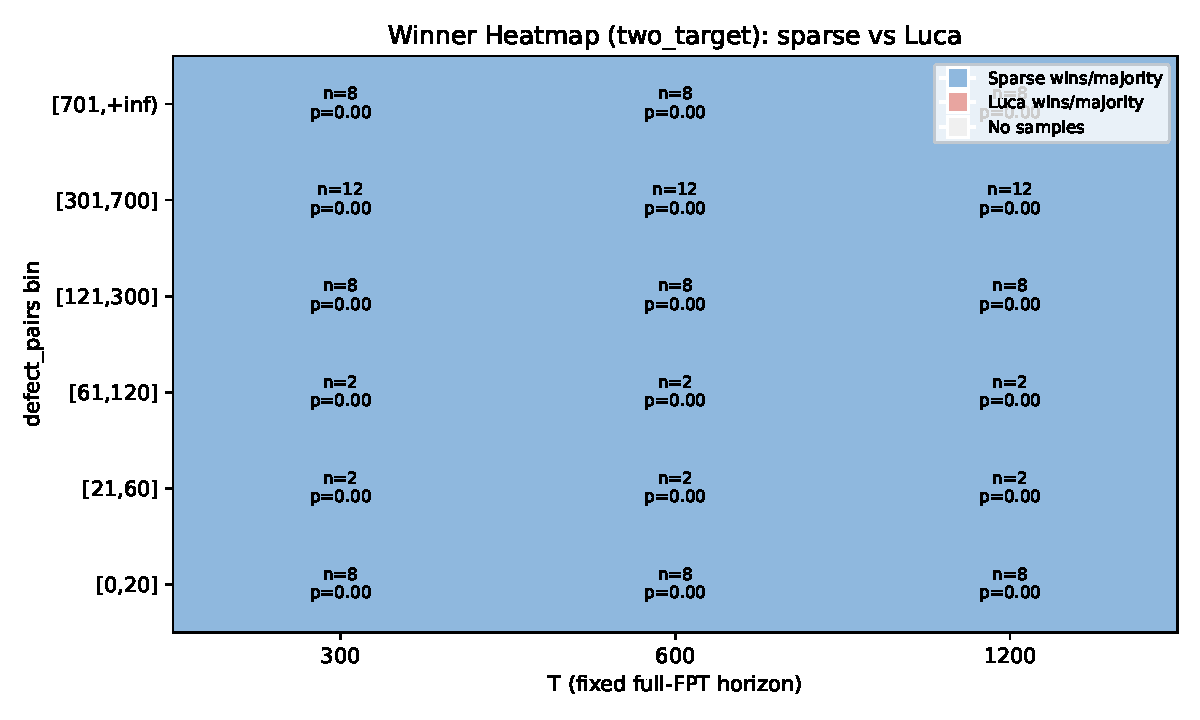
\includegraphics[width=0.9\linewidth]{figures/regime_winner_heatmap_two_target.pdf}
\caption{Winner heatmap on two-target workloads.}
\end{figure}
\begin{figure}[H]\centering
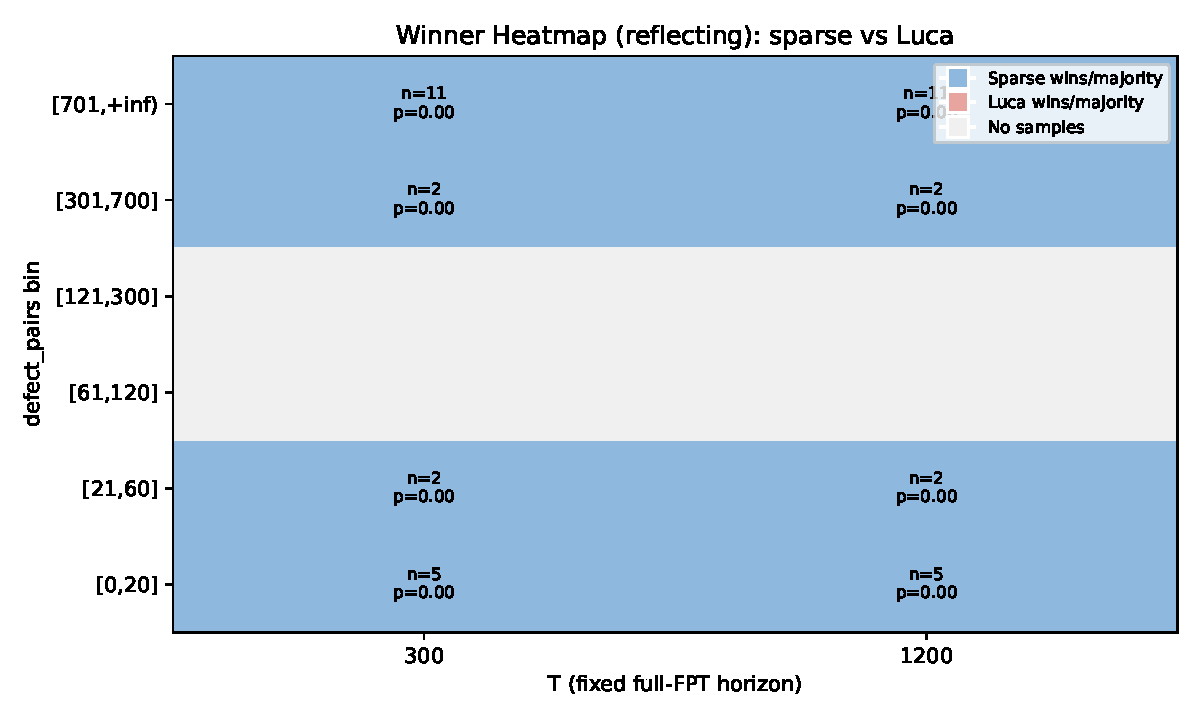
\includegraphics[width=0.9\linewidth]{figures/regime_winner_heatmap_reflecting.pdf}
\caption{Winner heatmap on reflecting workloads.}
\end{figure}
\begin{figure}[H]\centering
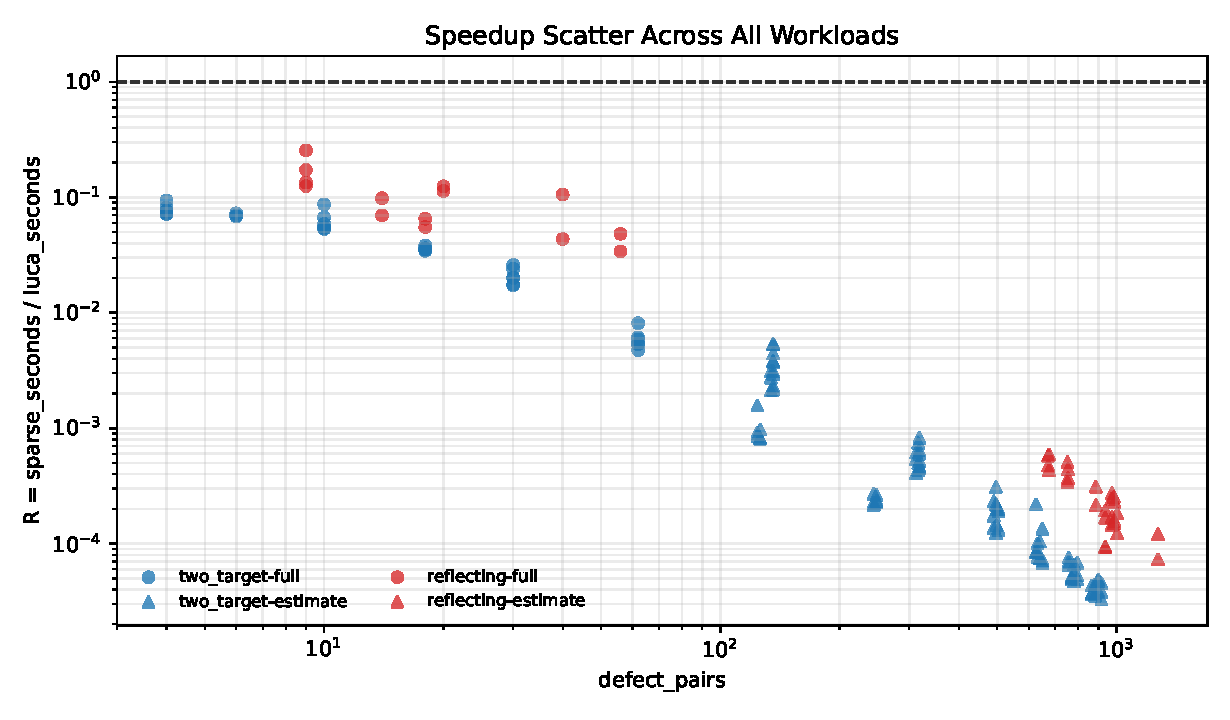
\includegraphics[width=0.9\linewidth]{figures/regime_speedup_scatter_all.pdf}
\caption{Speedup ratio scatter with full/estimate mode markers.}
\end{figure}
\begin{figure}[H]\centering
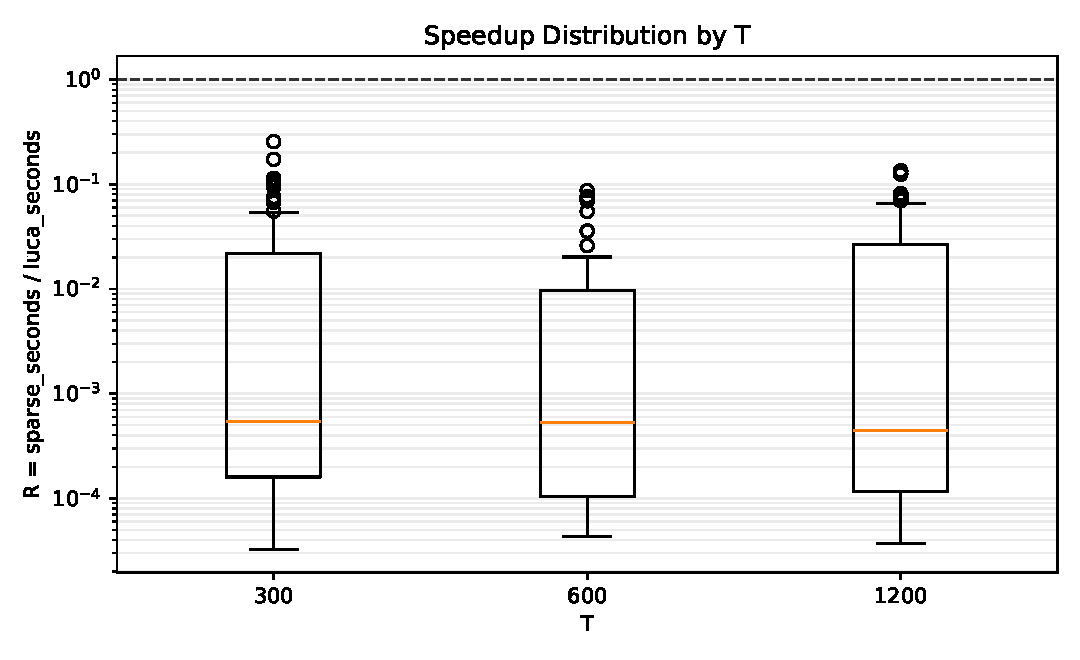
\includegraphics[width=0.8\linewidth]{figures/regime_speedup_box_by_T.pdf}
\caption{Distribution of $R$ by fixed horizon $T$.}
\end{figure}
\begin{figure}[H]\centering
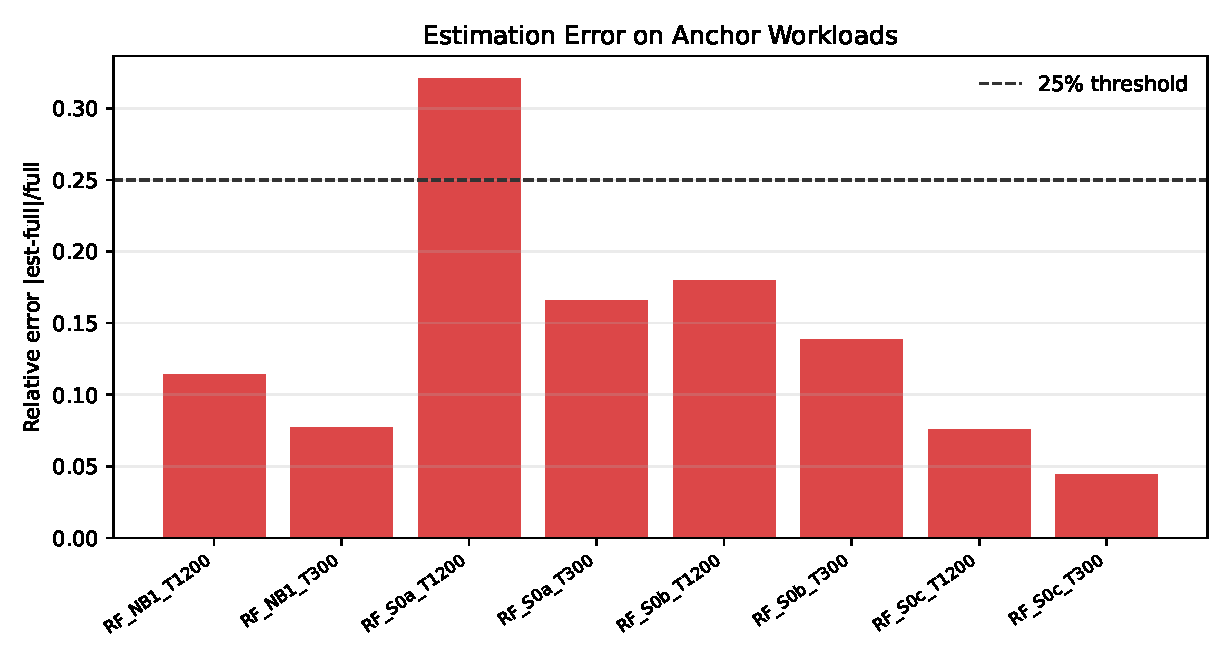
\includegraphics[width=0.8\linewidth]{figures/regime_estimation_error_anchor.pdf}
\caption{Full vs estimate relative error on anchor workloads.}
\end{figure}
\begin{figure}[H]\centering
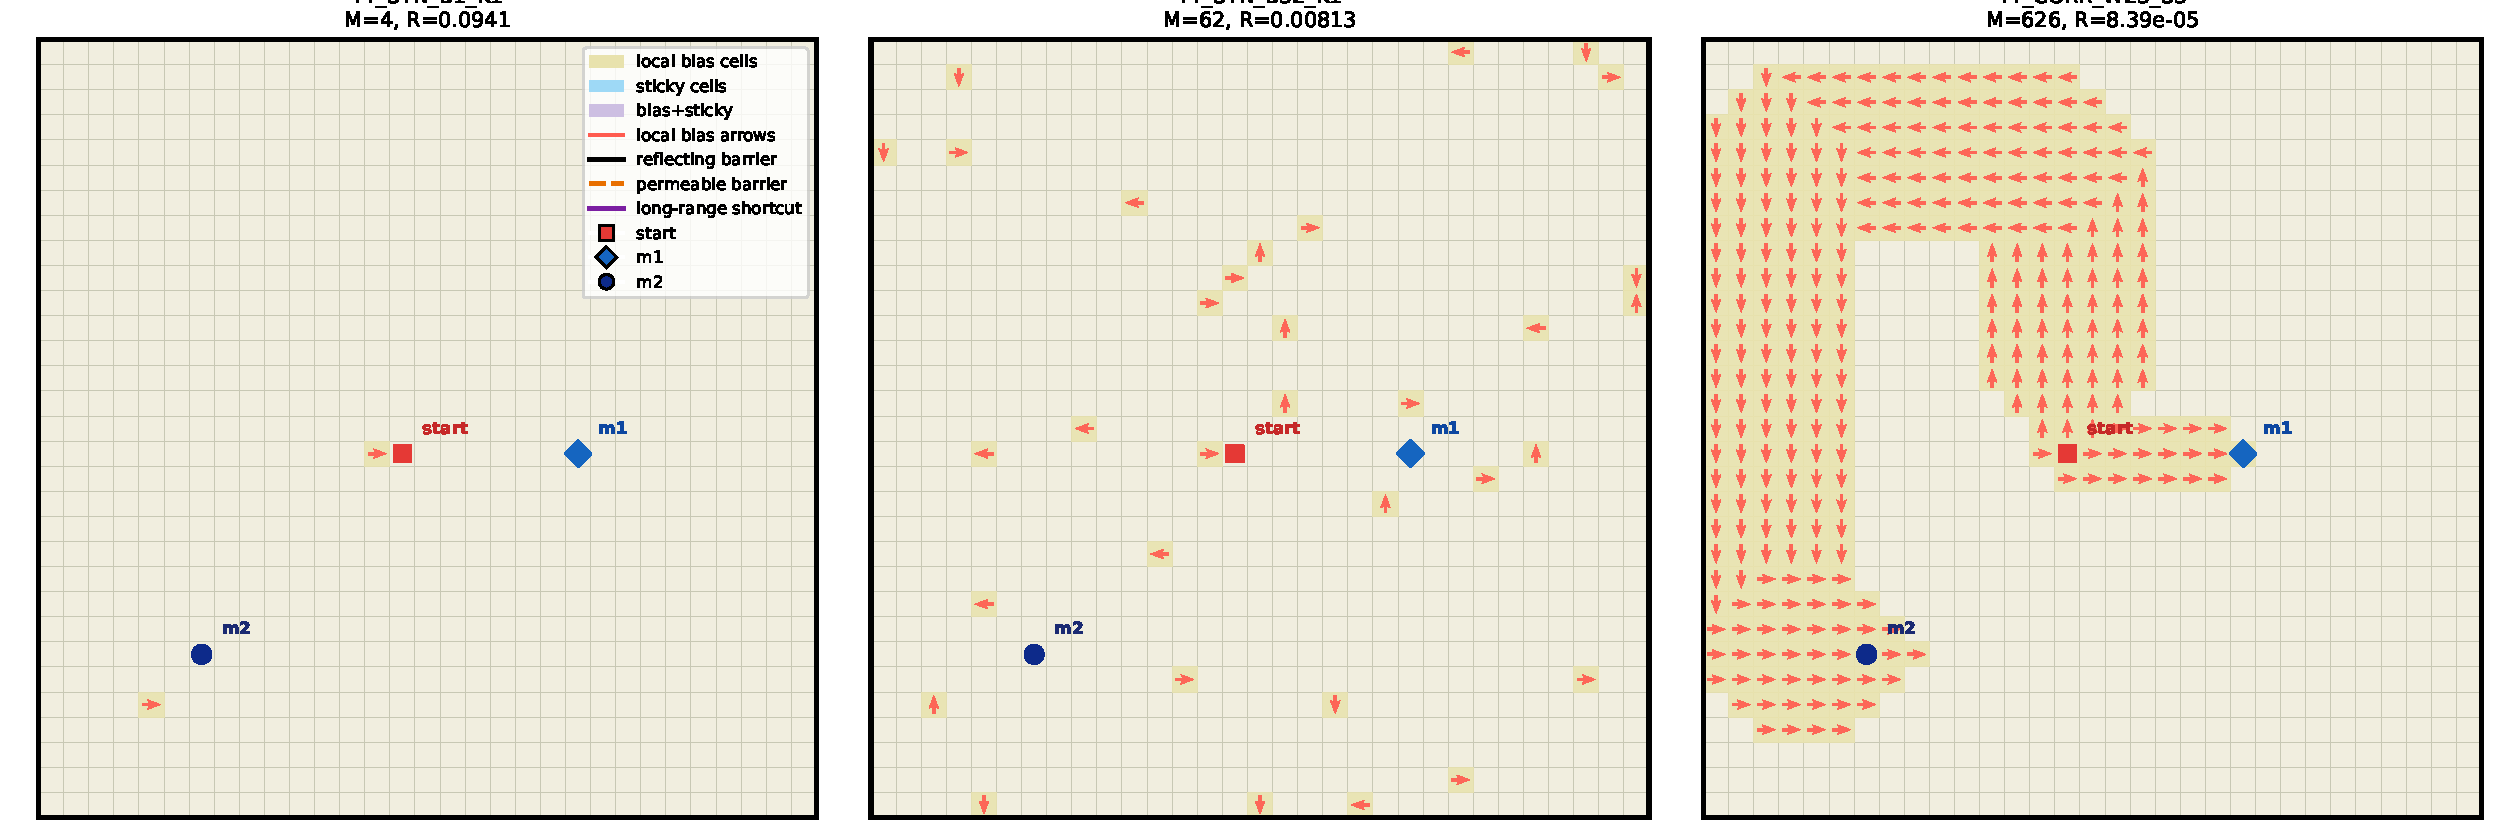
\includegraphics[width=0.98\linewidth]{figures/regime_config_examples.pdf}
\caption{Representative low/medium/high-defect configuration examples.}
\end{figure}
\section{Tables}
\begin{table}[H]
\centering
\small
\caption{Runtime ratio summary by defect bin and horizon.}
\resizebox{\linewidth}{!}{\begin{tabular}{lccccc}
\toprule
Defect bin & T & n & Median $R$ & Mean $R$ & $P(R>1)$ \\
\midrule
\texttt{[0,20]} & 300 & 13 & 0.0734 & 0.0919 & 0.000 \\
\texttt{[0,20]} & 600 & 8 & 0.0705 & 0.0628 & 0.000 \\
\texttt{[0,20]} & 1200 & 13 & 0.0727 & 0.0779 & 0.000 \\
\texttt{[121,300]} & 300 & 8 & 0.0019 & 0.0021 & 0.000 \\
\texttt{[121,300]} & 600 & 8 & 0.0015 & 0.0019 & 0.000 \\
\texttt{[121,300]} & 1200 & 8 & 0.0020 & 0.0021 & 0.000 \\
\texttt{[21,60]} & 300 & 4 & 0.0329 & 0.0472 & 0.000 \\
\texttt{[21,60]} & 600 & 2 & 0.0231 & 0.0231 & 0.000 \\
\texttt{[21,60]} & 1200 & 4 & 0.0290 & 0.0304 & 0.000 \\
\texttt{[301,700]} & 300 & 14 & 0.0002 & 0.0003 & 0.000 \\
\texttt{[301,700]} & 600 & 12 & 0.0002 & 0.0003 & 0.000 \\
\texttt{[301,700]} & 1200 & 14 & 0.0003 & 0.0003 & 0.000 \\
\texttt{[61,120]} & 300 & 2 & 0.0068 & 0.0068 & 0.000 \\
\texttt{[61,120]} & 600 & 2 & 0.0057 & 0.0057 & 0.000 \\
\texttt{[61,120]} & 1200 & 2 & 0.0053 & 0.0053 & 0.000 \\
\texttt{[701,+inf)} & 300 & 19 & 0.0002 & 0.0002 & 0.000 \\
\texttt{[701,+inf)} & 600 & 8 & 0.0000 & 0.0001 & 0.000 \\
\texttt{[701,+inf)} & 1200 & 19 & 0.0001 & 0.0001 & 0.000 \\
\bottomrule
\end{tabular}
}
\end{table}
\begin{table}[H]
\centering
\small
\caption{Anchor workload runtime baselines.}
\resizebox{\linewidth}{!}{\begin{tabular}{lcccccc}
\toprule
Anchor & Defects & Sparse(s) & Dense(s) & Full AW(s) & Luca(s) & Linear(s) \\
\midrule
low\_defect (TT\_SYN\_B1\_K1\_T300) & 4 & 0.0029 & 0.0050 & 22.9998 & 0.0416 & 0.0147 \\
high\_defect (TT\_CORR\_W23\_S2\_T300) & 632 & 0.0034 & 0.0065 & 22.2596 & 36.4872 & 0.0168 \\
\bottomrule
\end{tabular}
}
\end{table}
\section{Practical Recommendation Matrix}
\begin{table}[H]
\centering
\small
\begin{tabular}{@{}l>{\raggedright\arraybackslash}p{0.54\linewidth}@{}}
\toprule
Task Type & Recommended Method \\
\midrule
Full FPT under fixed finite horizon & Sparse exact recursion as default baseline; Luca only when defect support is very small and validated on anchors. \\
MFPT/splitting only & Linear systems (do not use as full-FPT winner metric). \\
Transform-domain analysis with sparse defects & Luca defect-reduced AW, but keep estimation/full calibration checks. \\
High-defect corridor-like regimes & Prefer sparse recursion; Luca often loses after setup/evaluation overhead is counted. \\
\bottomrule
\end{tabular}
\end{table}
\section{Reproducibility}
Core data files: \path{data/manifest.csv}, \path{data/runtime_raw.csv}, \path{data/runtime_summary.json}.
\end{document}
